\chapter{Introduction.}
Free probability is a non-commutative probability theory, introduced by Voiculescu in the 1980's.
While probability theory concerns itself with studying random variables -- measurable functions on a probability space -- non-commutative probability attempts to describe phenomena exhibited in algebras of non-commutative random variables, which are $*$-algebras equipped with positive states.
The original motivations for developing free probability related to the study of von Neumann algebras, but it has since been connected to other fields, such as random matrix theory and combinatorics.
The theory of free probability has been developed through both analytic and combinatorial techniques, and the interplay between these two has has led to many beautiful results.

\paragraph{Conventions.}
We will adopt the following conventions and notation:
\begin{itemize}
	\item We take inner products to be linear in the second entry and conjugate linear in the first.
	\item Given $n \in \N$, we will denote by $[n]$ the $n$-element set $\set{1, 2, \ldots, n}$.
	\item Unless we explicitly state otherwise, all algebras are unital $*$-algebras and all sub-algebras include the unit of the larger algebra.
\end{itemize}

\section{Preliminaries.}
We will provide a brief review of several ideas essential to free probability, which will be of use to us later on.
First, though, we will provide a lens through which probability theory may be viewed, which clarifies several analogies to free probability.


\subsection{Probability.}
To begin, we will recall some basics of probability.
Our presentation will differ from the usual, in order to make the generalisation to the free setting more natural.
Suppose that $(\Omega, \mathcal{F}, \P)$ is a probability space (so $\Omega$ is a set, $\cF$ is a $\sigma$-algebra on $\cF$, and $\P$ is a positive measure of total mass $1$), and let $\A = L^\infty(\Omega, \P)$ be the algebra of essentially bounded functions on $\Omega$ (i.e., the algebra of bounded random variables on $\Omega$).
Then $\A$ can be embedded in the bounded operators on the Hilbert space $L^2(\Omega, \P)$ via pointwise multiplication.
Notice that the expectation function $\E : \A \to \C$ can be extended to $B(L^2(\Omega, \P))$ as the vector state corresponding to $1 \in L^2(\Omega, \P)$: for any $X \in \A$,
$$\E[X] = \ang{1, X(1)}.$$
We will often forget the underlying probability space $(\Omega, \P)$ and consider normed commutative unital $*$-algebras equipped with states (i.e., positive linear functionals which map $1_\A$ to $1$); overloading terminology, we will also refer to such a pair as a probability space.

Recall that subalgebras $(\A^{(\iota)})_{\iota\in\I}$ are independent if for any $X_1, \ldots, X_n \in \A$ with $X_k \in \A^{(i_k)}$ such that $i_1, \ldots, i_n$ are distinct, we have the identity
$$\E[X_1\cdots X_n] = \E[X_1]\cdots\E[X_n].$$
Notice that it is equivalent to ask that this identity holds only for $\oX_1, \ldots, \oX_n$ when $\E[\oX_k] = 0$ for each $k$.
Indeed, given arbitrary $X_1, \ldots, X_n$, we can set $\oX_j = X_j - \E[X_j]$ and obtain the relation by expanding the multiplication in
$$\E\sq{\oX_1\cdots\oX_n} = 0.$$
Random variables are then said to be independent if they generate independent subalgebras of $\A$.
Note that the value of $\E$ on the algebra generated by the $(\A^{(\iota)})_{\iota\in\I}$ is completely prescribed by its values on the individual $\A^{(\iota)}$ and the condition that they be independent.
In fact, our condition for independence still makes sense and still prescribes joint moments in terms of pure ones if we take $\A^{(\iota)} \subset \A$ which commute with one another, but may not themselves be commutative!

%Algebras of random variables may always be embedded into a larger algebra in a manner which makes them independent.
%The usual approach is to take products on the level of probability spaces; however, we can also perform such a construction on the level of Hilbert spaces.
%Suppose therefore that we have $\A^{(\iota)} \subset L^\infty(\Omega^{(\iota)}, \P^{(\iota)}) \subset B(L^2(\Omega^{(\iota)}, \P^{(\iota)})$ for each $\iota \in \I$, and for simplicity assume $\I = \set{1, \ldots, n}$ is finite.
%Then if we set $\Hi = L^2(\Omega^{(1)}, \P^{(1)}) \otimes \cdots\otimes L^2(\Omega^{(n)}, \P^{(n)})$ and define $\E : B(\Hi) \to \C$ by $\E[X] = \ang{1, X(1)}$ (where by $1$ we mean the tensor product of the constant function in each $L^2$ space), we find that the algebras $1\otimes\cdots\otimes1\otimes \A^{(j)}\otimes 1 \otimes\cdots\otimes 1$ are independent and isomorphic to the original $\A^{(j)}$.
%
Algebras of random variables may always be embedded into a larger algebra in a manner which makes them independent.
The usual approach is to take products on the level of probability spaces $(\Omega, \cF, \P)$; however, since we have forgotten the underlying probability space, this is not possible in our context.
We will perform the construction in a more complicated manner, which will be easily duplicated in the non-commutative case.

A vector space with specified state vector is a triple $(V, \oV, \xi)$ where $V$ is a vector space such that $V = \oV\oplus\C\xi$.
We define a state $\varphi_\xi$ on $L(V)$, the space of linear operators on $V$, by taking $\varphi_\xi(T)$ to be the unique element of $\C$ so that $T(\xi) \in \oV + \varphi_\xi(T)\xi$.
This makes $(L(V), \varphi_\xi)$ into a probability space (and any probability space $(\A, \E)$ can be realized in this form by letting $V = \A$, $\xi = 1_\A$, and $\oV = \ker\E$, then having $\A$ act on $V$ by multiplication).
Now suppose that for each $\iota \in \I$ we have $\A^{(\iota)} \subset L(V^{(\iota)})$ with state vectors $\xi^{(\iota)}$; for simplicity, assume $\I = \set{1, \ldots, n}$ is finite.
Consider the space $V = V^{(1)}\otimes\cdots\otimes V^{(n)}$ and let $\xi = \xi^{(1)}\otimes\cdots\otimes\xi^{(n)}$, with $\oV = \operatorname{span}_{j\in\I}\paren{\oV^{(j)}\otimes\bigotimes_{\iota\neq j}V^{(\iota)}}$; note that $\varphi_\xi = \varphi_{\xi^{(1)}}\otimes\cdots\otimes\varphi_{\xi^{(n)}}$.
Then $\A^{(\iota)}$ embeds in $L(V)$ as $1\otimes\cdots\otimes1\otimes \A^{(\iota)} \otimes1\otimes\cdots\otimes1$ in a state preserving way, and these embeddings are independent from one another under $\varphi_\xi$.

This gives us another way of recognising independence: subalgebras $(\A^{(\iota)})_{\iota\in\I}$ of $(\A, \varphi)$ are independent if there exist vector spaces with specified state vectors $(V^{(\iota)}, \oV^{(\iota)}, \xi^{(\iota)})$ and embeddings $\rho^{(\iota)} : \A^{(\iota)} \to L(V^{(\iota)})$ such that the following diagram commutes:
	\[\begin{tikzpicture}
		\node (q) at (-3, 1.2) {$\displaystyle\bigotimes_{\iota\in\I}\A^{(\iota)}$};
		\node (a) at (-3, -1.2) {$L\paren{\displaystyle\bigotimes_{\iota\in\I}V^{(\iota)}}$};
		\node (w) at (3, 1.2) {$\A$};
		\node (s) at (3, -1.2) {$\C$};
		\node at (0,0) {$\circlearrowleft$};

		\draw [->] (q) -- node[above] {$\operatorname{ev}$} (w);
		\draw [->] (q) -- node[left] {$\bigotimes_{\iota\in\I}\rho^{(\iota)}$} (a);
		\draw [->] (a) -- node[above] {$\varphi_\xi$} (s);
		\draw [->] (w) -- node[right] {{$\varphi$}} (s);
	\end{tikzpicture}\]

\subsection{Free probability.}
\label{ssec:freeind}
We will be working in the context of a non-commutative algebra, so it will be useful to have some operator algebraic concepts.
A (concrete unital) $C^*$-algebra is a $*$-subalgebra of $B(\cH)$ containing the identity operator which is closed under the operator norm topology.
A (concrete) von Neumann algebra is a $*$-subalgebra of $B(\cH)$ which is closed under the weak operator topology, or equivalently is closed under the strong operator topology, or equivalently is equal to its own bicommutant: that is, if $\A' \subset B(\cH)$ is defined as $\set{x \in B(\cH) : xa = ax\,\forall a \in \A}$, a von Neumann algebra satisfies $\A'' = \A$.
A von Neumann algebra is called a factor if its centre is $\C1$.
A state on a $*$-algebra $\A$ is a linear map $\varphi : \A \to \C$ such that $\varphi(1) = 1$ and $\varphi$ is positive in the sense that $\varphi(a^*a) \geq 0$ for $a \in \A$.
A state is
\begin{itemize}
	\item faithful if $\varphi(a*a) = 0$ implies $a = 0$;
	\item normal if for every bounded increasing net $a_\alpha \to a$, $\varphi(a) = \lim_{\alpha}\varphi(a_\alpha)$; and
	\item tracial if $\varphi(ab) = \varphi(ba)$.
\end{itemize}
When we deal with von Neumann algebras, we will usually assume that they are finite (in the sense that no projection is equivalent to a proper subprojection) and equipped with faithful normal tracial states.
A finite factor which is not isomorphic to $B(\cH)$ and admits a faithful normal tracial state is said to be of type $\mathrm{II}_1$.

A non-commutative probability space is a pair $(\A, \varphi)$ where $\A$ is a unital $*$-algebra and $\varphi : \A \to \C$ is a state.
Elements of $\A$ can be thought of as non-commutative random variables.
Note that we make no assumption that $\A$ is non-commutative, so $L^\infty(\Omega, \P)$ is a non-commutative probability space; the ``non-commutative'' merely references the potential of $\A$ to contain elements which do not commute, in much the same way that ``densely-defined unbounded operators'' may be defined everywhere and bounded.

Suppose that $\A$ is a $C^*$-algebra, and $x \in \A$ is normal.
Then by Gelfand duality, the $C^*$-algebra generated by $x$ is isometrically isomorphic to the continuous functions on the (compact) spectrum of $x$, which when coupled with the spectral measure of $x$ becomes a probability space.
Thus normal elements of $C^*$ non-commutative probability spaces are random variables in a very concrete sense.
Given a collection of elements $x_1, \ldots, x_n \in \A$, their law is the map
$$\mu_{(x_1, \ldots, x_n)} : \C\ang{X_1, \ldots, X_n} \to \C$$
given by $\mu_{(x_1, \ldots, x_n)}(P(X_1, \ldots, X_n)) = \varphi(P(x_1, \ldots, x_n))$.
When $x_1, \ldots, x_n$ are commuting normal elements of a $C^*$ algebra, this corresponds to their joint law in the usual probability sense.

We are now ready to introduce free independence as a non-commutative analogue of independence, using the final picture of independence as our starting point.
For this we introduce the free product of vector spaces with specified state vectors, an analogue to the tensor product in much the same way that the free product of groups is a non-commutative analogue of their direct product.
Given a collection $(V^{(\iota)}, \oV^{(\iota)}, \xi^{(\iota)})_{\iota\in\I}$ of vector spaces with specified state vectors (so once again $V^{(\iota)} = \oV^{(\iota)}\oplus\C\xi^{(\iota)}$) we define their free product to be the triple $(V, \oV, \xi)$ where $V = \oV\oplus\C\xi$ and
$$\oV := \bigoplus_{n \geq 1}\bigoplus_{i_1\neq i_2 \neq \cdots \neq i_n} \oV^{(i_1)} \otimes \cdots \otimes \oV^{(i_n)}.$$
Here the condition $i_1\neq i_2\neq \cdots \neq i_n$ requires only that \emph{adjacent} indices be unequal.
We denote $\displaystyle\st_{\iota\in\I}V^{(\iota)} := V$ and $\displaystyle\st_{\iota\in\I}\xi^{(\iota)} := \xi$.

Suppose $V = \st_{\iota\in\I}V^{(\iota)}$; then we can embed $L(V^{(i)})$ in $L\paren{V}$ as follows.
First, we define
$$V(\ell, j) := \C\xi \oplus\bigoplus_{n\geq1}\bigoplus_{j\neq i_1\neq \cdots\neq i_n}\oV^{(i_1)}\otimes\cdots\otimes\oV^{(i_n)}.$$
The space $V(\ell, j)$ can be thought of as words in $V$ which do not begin with a letter from $\oV^{(j)}$.
Then we have $V^{(j)}\otimes V(\ell, j) \cong V$ via the map $W_j$ which makes the obvious identifications:
\begin{align*}
	W_j(\xi^{(j)}\otimes\xi) &= \xi \\
	W_j(\xi\otimes(\oV^{(i_1)}\otimes\cdots\otimes\oV^{(i_n)})) &= \oV^{(i_1)}\otimes\cdots\otimes\oV^{(i_n)} \\
	W_j(\oV^{(j)}\otimes\xi) &= \oV^{(j)} \\
	W_j(\oV^{(j)}\otimes(\oV^{(i_1)}\otimes\cdots\otimes\oV^{(i_n)})) &= \oV^{(j)}\otimes\oV^{(i_1)}\otimes\cdots\otimes\oV^{(i_n)}.
\end{align*}
This gives us a left representation $\lambda^{(\iota)} : L(V^{(j)}) \to L(V)$ via $\lambda^{(\iota)}(T) = W_j\circ(T\otimes 1)\circ W_j^{-1}$.
Note that we may perform a similar decomposition by factoring $V^{(j)}$ out of $V$ on the right, say $U_j : V(r, j)\otimes V^{(j)} \to V$ (where $V(r, j)$ is defined analogously to be words which do not end with a letter from $V^{(j)}$), and produce a right representation on the free product via $\rho^{(\iota)}(T) = U_j\circ(1\otimes T)\circ U_j^{-1}$.


Now, given $*$-subalgebras $(\A^{(\iota)})_{\iota\in\I}$ of a non-commutative probability space $(\A, \varphi)$, we say they are \emph{freely independent} (or \emph{free}) if there exist vector spaces with specified state vectors $(V^{(\iota)}, \oV^{(\iota)}, \xi^{(\iota)})$ and embeddings $\pi^{(\iota)} : \A^{(\iota)} \to L(V^{(\iota)})$ such that the following diagram commutes:
	\[\begin{tikzpicture}
		\node (q) at (-3, 1.2) {$\displaystyle\st_{\iota\in\I}\A^{(\iota)}$};
		\node (a) at (-3, -1.2) {$L\paren{\displaystyle\st_{\iota\in\I}V^{(\iota)}}$};
		\node (w) at (3, 1.2) {$\A$};
		\node (s) at (3, -1.2) {$\C$};
		\node at (0,0) {$\circlearrowleft$};

		\draw [->] (q) -- node[above] {$\operatorname{ev}$} (w);
		\draw [->] (q) -- node[left] {$\st_{\iota\in\I}\lambda^{(\iota)}\circ\pi^{(\iota)}$} (a);
		\draw [->] (a) -- node[above] {$\varphi_\xi$} (s);
		\draw [->] (w) -- node[right] {{$\varphi$}} (s);
	\end{tikzpicture}\]
Here $\st_{\iota\in\I}\A^{(\iota)}$ we mean the formal algebraic free product consisting of reduced words with letters coming from the $\A^{(\iota)}$, and by $\st_{\iota\in\I}\lambda^{(\iota)}\circ\pi^{(\iota)}$ we mean the unique algebra homomorphism which is $\lambda^{(\iota)}\circ\pi^{(\iota)}$ when restricted to $\A^{(\iota)}$.
Notice that given a family of algebras $(\A^{(\iota)})_{\iota\in\I}$ we can use this construction to produce a state on their algebraic free product with respect to which they are free.

\begin{example}
	\label{ex:freegroupsarefree}
	Suppose that $\Gamma_1, \ldots, \Gamma_n$ are countable groups and $\Gamma = \Gamma_1\st\cdots\st\Gamma_n$.
	Let $\tau : \C[\Gamma] \to \C$ be the linear functional given by $\tau(e) = 1$ and $\tau(g) = 0$ for other $g \in \Gamma$.
	Then $(\C[\Gamma], \tau)$ is a non-commutative probability space, and the family of algebras $\paren{\C[\Gamma_i]}_{i=1}^n$ are freely independent.
	Notice that $\C[\Gamma]$ can be represented on $\ell^2(\Gamma)$ via left translation, and $\tau(x) = \ang{\delta_0, x\cdot\delta_0}$.
\end{example}

Unfortunately, this is not a very practical condition for checking free independence.
Fortunately, it can be reformulated in terms of conditions on mixed moments which are far more approachable.
\begin{proposition}
\label{prop:freemomentsvanish}
	Suppose $(\A^{(\iota)})_{\iota\in\I}$ is a family of unital $*$-subalgebras of a non-commutative probability space $(\A, \varphi)$.
	Then the family is freely independent if and only if whenever $a_1, \ldots, a_n \in \A$ are such that $a_j \in \A^{(i_j)}$ with $i_1 \neq i_2\neq \cdots \neq i_n$ and $\varphi(a_j) = 0$ for each $j$, we have $\varphi(a_1\cdots a_n) = 0$.
	That is, if and only if alternating products of centred variables are centred.
\end{proposition}

\begin{proof}
	Suppose $(\A^{(\iota)})_{\iota\in\I}$ are free, with their freeness realised via $\st_{\iota\in\I}V^{(\iota)}$, and let $a_1, \ldots, a_n$ be as in the statement of the proposition.
	Notice that $v_n := \lambda^{(i_n)}\circ\pi^{(i_n)}(a_n)\xi \in \oV^{(i_n)}$ as $\varphi(a_n) = 0$.
	Similarly, $v_{n-1} := \lambda^{(i_{n-1})}\circ\pi^{(i_{n-1})}(a_{n-1})v_n \in \oV^{(i_{n-1})}\otimes \oV^{(i_n)}$ since $\varphi(a_{n-1}) = 0$.
	Continuing this in the obvious manner, we find $v_1 \in \oV^{(i_1)}\otimes\cdots\otimes\oV^{(i_n)}$ and hence
$$\varphi_\xi\paren{\st_{\iota\in\I}\lambda^{(\iota)}\circ\pi^{(\iota)}\paren{a_1\cdots a_n}} = 0.$$

	Now, on the other hand, suppose that all alternating products of centred variables are themselves centred.
	Notice that this determines all mixed moments in terms of pure moments from the families: given arbitrary $b_1, \ldots, b_n$ with $b_j \in \A^{(i_j)}$ and $i_1 \neq i_2\neq\cdots\neq i_n$, we find
	$$\varphi\paren{(b_1-\varphi(b_1))\cdots(b_n-\varphi(b_n))} = 0;$$
	expanding this gives us an equation for $\varphi(b_1\cdots b_n)$ in terms of products of mixed moments with fewer terms, which may themselves be recursively reduced to pure moments.
	%Thus there is a unique state on the algebra generated by the $\A^{(\iota)}$ which satisfies this condition.
	%However, if we 
	Thus there is a unique state on $\st_{\iota\in\I}\A^{(\iota)}$ which satisfies this condition.
	However, if we let $\mu$ be the state on $\st_{\iota\in\I}\A^{(\iota)}$ which makes the individual algebras free, we find $\mu$ satisfies the alternating moment condition by the first part of this argument.
	Then by uniqueness, $\mu$ is equal to $\varphi$ and so the $(\A^{(\iota)})_{\iota\in\I}$ are free with respect to $\varphi$.
\end{proof}

\subsection{Free cumulants.}
	The free cumulants were introduced by Speicher to better understand the combinatorics of free independence, and free additive convolution \cite{speicher1997free,speicher1994}.

\begin{definition}
	A \emph{partition} of a finite set $S$ is a set $\pi = \set{B_1, \ldots, B_n}$ of non-empty subsets of $S$ which are pairwise disjoint with $S = \bigcup_{i=1}^n B_i$.
	The sets $B_i$ are referred to as the \emph{blocks} of $\pi$.
	For $x, y \in S$ we write $x \sim_\pi y$ if there is some $B \in \pi$ with $x \in B, y \in B$.
	We define $\cP(n) := \set{\pi : \pi \text{ is a partition of } [n]}$.

	A partition $\pi \in \cP(n)$ is said to be \emph{non-crossing} if whenever $1 \leq i < j < k < \ell \leq n$ are such that $i \sim_\pi k$ and $j \sim_\pi \ell$, we have $j \sim_\pi k$.
	The set of non-crossing partitions of $n$ elements is denoted $\NC(n) := \set{\pi \in \cP(n) : \pi \text{ is non-crossing}}$.
\end{definition}
Non-crossing partitions are so named because they are exactly those which can be diagrammatically represented above the number line without needing to draw crossing blocks.

\begin{example}
	There are 15 elements in $\cP(4)$, of which 14 are non-crossing.
	\[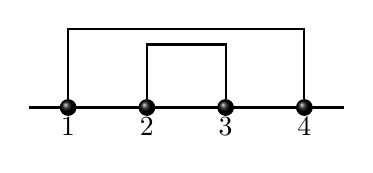
\begin{tikzpicture}[baseline]
		\foreach \y in {1, ..., 4} {
			\draw [thick] (\y-0.5,0) -- node [midway, below] {\y} ++(1,0);
			\node (ball\y) [draw, shade, circle, ball color=black, inner sep=0.07cm] at (\y, 0) {};
		}
		\draw [thick] (ball1) -- ++(0, 1) -| (ball4);
		\draw [thick] (ball2) -- ++(0, 0.8) -| (ball3);
	\end{tikzpicture} \qquad
	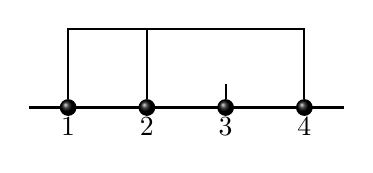
\begin{tikzpicture}[baseline]
		\foreach \y in {1, ..., 4} {
			\draw [thick] (\y-0.5,0) -- node [midway, below] {\y} ++(1,0);
			\node (ball\y) [draw, shade, circle, ball color=black, inner sep=0.07cm] at (\y, 0) {};
		}
		\draw [thick] (ball1) -- ++(0, 1) -| (ball4);
		\draw [thick] (ball2) -- ++(0, 1);
		\draw [thick] (ball3) -- ++(0, 0.3);
	\end{tikzpicture} \qquad
	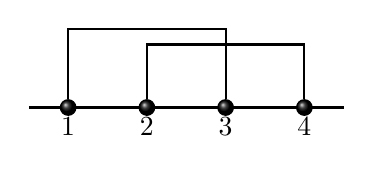
\begin{tikzpicture}[baseline]
		\foreach \y in {1, ..., 4} {
			\draw [thick] (\y-0.5,0) -- node [midway, below] {\y} ++(1,0);
			\node (ball\y) [draw, shade, circle, ball color=black, inner sep=0.07cm] at (\y, 0) {};
		}
		\draw [thick] (ball1) -- ++(0, 1) -| (ball3);
		\draw [thick] (ball2) -- ++(0, 0.8) -| (ball4);
	\end{tikzpicture}\]
The partitions $\set{\set{1, 4}, \set{2, 3}}$ and $\set{\set{1,2,4}, \set{3}}$ are non-crossing, while $\set{\set{1,3}, \set{2,4}}$ is the only element of $\cP(4)$ which is not non-crossing.
\end{example}

The set $\cP(n)$ is partially ordered by refinement: given $\pi, \sigma \in \cP(n)$ we say $\sigma$ \emph{refines} $\pi$, and write $\sigma \prec \pi$, if every block of $\pi$ is a union of blocks of $\sigma$.
This ordering makes $\cP(n)$ into a lattice with minimum element $\set{\set{1}, \ldots, \set{n}}$ and maximum element $\set{[n]}$, denoted respectively $0_{\cP(n)}$ and $1_{\cP(n)}$ (although when context makes it clear we may instead write $0_n$ and $1_n$).

We are now ready to define the free cumulants.
\begin{definition}
	Suppose $(\A, \varphi)$ is a non-commutative probability space.
	The \emph{free cumulants} are a family of linear functionals $(\kappa_n)_{n\geq 1}$ with $\kappa_n : \A^n \to \C$ defined recursively by the \emph{moment-cumulant formula}: for any $a_1, \ldots, a_n \in \A$,
	$$\varphi(a_1\cdots a_n) = \sum_{\pi\in\NC(n)}\prod_{\set{i_1 < \cdots < i_k} \in \pi}\kappa_{k}\paren{a_{i_1}, \ldots, a_{i_k}}.$$
	Here the product is taken over the blocks of $\pi$.
\end{definition}
	We may denote the product appearing in this relation as $\kappa_\pi(a_1, \ldots, a_n)$ when it is convenient to do so, and given $B = \set{i_1 < \cdots < i_k} \subset [n]$ we may abbreviate $\kappa_k(a_{i_1}, \ldots, a_{i_k}) =: \kappa_k(a_B)$.
	%Likewise, it will often be convenient to write $\varphi_\pi(a_1, \ldots, a_n) := \prod_{\set{i_1 < \cdots < i_k}\in\pi} \varphi(a_{i_1}\cdots a_{i_k})$, and similarly, $\varphi(a_B) := \varphi(a_{i_1}\cdots a_{i_k})$.
	Likewise, it will often be convenient to write
	$$\varphi(a_B) := \varphi(a_{i_1}\cdots a_{i_k}) \qquad\text{ and }\qquad \varphi_\pi(a_1, \ldots, a_n) := \prod_{B\in\pi} \varphi(a_B).$$

\begin{theorem}[\cite{speicher1994}]
	\label{thm:cumufree}
	Let $(\A^{(\iota)})_{\iota\in\I}$ be subalgebras of a non-commutative probability space $(\A, \varphi)$.
	Then $(\A^{(\iota)})_{\iota\in\I}$ are free if and only if all mixed cumulants vanish, i.e., whenever $a_1, \ldots, a_n \in \A$ with $a_j \in \A^{(i_j)}$ and $i_j \neq i_k$ for some $j, k$, we have
	$$\kappa_n(a_1, \ldots, a_n) = 0.$$
\end{theorem}

\subsection{The incidence algebra of non-crossing partitions.}
To better understand the cumulant functionals, Speicher in \cite{speicher1994} made a study of the incidence algebra of non-crossing partitions.
We provide an overview of some of those arguments, as they will provide a starting point for some of our arguments later on.

\begin{proposition}[\cite{speicher1994}*{Proposition 1}]
	\label{prop:ncfactoring}
	Suppose $\sigma\prec\pi \in \NC(n)$.
	Then there is a canonical decomposition of $[\sigma, \pi] := \set{\rho \in \NC(n) : \sigma\preceq\rho\preceq\pi}$ as a product of full lattices:
$$\prod_{j=1}^k \NC(a_j).$$
\end{proposition}

\begin{proof}[Sketch of proof]
	First, we notice that we may decompose the intervals into pieces corresponding to the blocks of $\pi$:
	$$[\sigma, \pi] \cong \prod_{B\in\pi} [\set{C \in \sigma : C \subset B}, \set{B}] \subset \prod_{B\in\pi} \NC(\# B).$$
	(Here we have abused notation slightly: $\set{B} \notin \NC(\#B)$ in general since the labels are wrong; this can be fixed in the obvious way, by relabeling with the numbers $1, \ldots, \#B$ while maintaining ordering.)

	Now, given an interval $[\sigma, 1_n]$, if possible we select a block $\set{i_1<\cdots<i_k} \in \sigma$ and $1 \leq j < k$ so that $i_j + 1 < i_{j+1}$.
	We then take
	\begin{align*}
		\sigma_0 &= \set{C \in \sigma : C \subset [n] \setminus\set{i_{j}+1, \ldots, i_{j+1}-1}},\\
		\sigma_1 &= \set{C \in \sigma : C \subset\set{i_{j}+1, \ldots, i_{j+1}-1}}.
	\end{align*}
	Note that the non-crossing condition ensures that every block of $\sigma$ is accounted for above.
	We now make the identification
	$$[\sigma, 1_n] \cong [\sigma_0, 1_{n-(i_{j+1}-i_j-1)}] \times [\sigma_1 \cup \set{\set{0}}, 1_{i_{j+1}-i_j}].$$
	We have added a dummy node to the right hand product to represent the block which is dividing the partition.
	The left hand interval here shoud be ignored if $\sigma_0 = 1_{n-(i_{j+1}-i_j-1)}$.
	
	This may be continued until we are left with a product of terms of the form $[\sigma, 1_n]$, with $\sigma$ consisting of intervals.
	But in this case, $[\sigma, 1_n] \cong \NC(\#\sigma)$.

	There is some potential ambiguity due to the fact that as lattices, $[\sigma, \pi] \cong \NC(1)\times[\sigma, \pi]$; we resolve this by insisting that we only take copies of $\NC(1)$ when the last step in the decomposition requires us to do so.
\end{proof}

\begin{example}
	\begin{align*}
	\sq{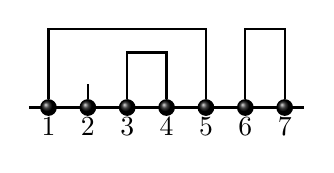
\begin{tikzpicture}[baseline,shift={(0, -0.3)}]
		\draw [thick] (0.25, 0) -- ++(3.5, 0);
		\foreach \y in {1, ..., 7} {
			\node (ball\y) [draw, shade, circle, ball color=black, inner sep=0.07cm] at (0.5*\y, 0) {};
			\node [below] at (ball\y) {\y};
		}
		\draw [thick] (ball1) -- ++(0, 1) -| (ball5);
		\draw [thick] (ball2) -- ++(0, 0.3);
		\draw [thick] (ball3) -- ++(0, 0.7) -| (ball4);
		\draw [thick] (ball6) -- ++(0, 1) -| (ball7);
	\end{tikzpicture}, 1_7}
	&\cong
	\sq{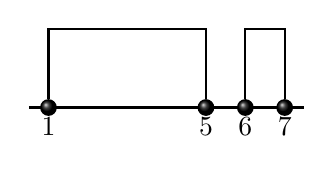
\begin{tikzpicture}[baseline,shift={(0, -0.3)}]
		\draw [thick] (0.25, 0) -- ++(3.5, 0);
		\foreach \y in {1, 5, 6, 7} {
			\node (ball\y) [draw, shade, circle, ball color=black, inner sep=0.07cm] at (0.5*\y, 0) {};
			\node [below] at (ball\y) {\y};
		}
		\draw [thick] (ball1) -- ++(0, 1) -| (ball5);
		\draw [thick] (ball6) -- ++(0, 1) -| (ball7);
	\end{tikzpicture}, 1_4}
	\times
	\sq{\begin{tikzpicture}[baseline,shift={(0, -0.3)}]
		\draw [thick] (0.25, 0) -- ++(3.5, 0);
		\foreach \y in {2, 3, 4} {
			\node (ball\y) [draw, shade, circle, ball color=black, inner sep=0.07cm] at (0.5*\y, 0) {};
			\node [below] at (ball\y) {\y};
		}
		\node (ball0) [draw, shade, circle, ball color=black, inner sep=0.07cm] at (0.5, 0) {};
		\node [below] at (ball0) {0};
		\draw [thick,dashed,black!50] (ball0) -- ++(0, 1) -| ($ (ball4) + (0.5, 0) $);
		\draw [thick] (ball2) -- ++(0, 0.3);
		\draw [thick] (ball3) -- ++(0, 0.7) -| (ball4);
	\end{tikzpicture}, 1_7}
	\\&\cong \NC(2) \times \NC(3)
	\end{align*}
\end{example}

The incidence algebra on the lattice of non-crossing partitions consists of the following set of functions:
$$IA(\NC) := \set{ f : \coprod_{n\geq1} \NC(n)\times\NC(n) \to \C \middle| f(\sigma, \pi) = 0 \text{ unless } \sigma\preceq\pi }.$$
We equip $IA(\NC)$ with the convolution product given as follows:
$$(f\star g)(\sigma, \pi) := \sum_{\sigma \leq \rho \leq \pi} f(\sigma, \rho)g(\rho, \pi).$$

\begin{definition}
	A function $f \in IA(\NC)$ is said to be \emph{multiplicative} if whenever $[\sigma, \pi] \cong \prod_{j=1}^k \NC(a_j)$ as in Proposition~\ref{prop:ncfactoring}, one has
	$$f(\sigma, \pi) = \prod_{j=1}^k f(0_{a_j}, 1_{a_j}).$$
\end{definition}
Notice that for a given sequence of numbers $(x_n)$, there is a unique multiplicative function so that $f(0_n, 1_n) = x_n$ for every $n$.

\begin{proposition}[\cite{speicher1994}*{Proposition 2}]
	\label{prop:mcmism}
	The convolution of two multiplicative functions is multiplicative.
\end{proposition}

\begin{proof}[Sketch of proof]
	Suppose $[\sigma, \pi] \cong \prod_{j=1}^k \NC(a_j)$.
	Then
	\begin{align*}
		(f\star g)(\sigma, \pi)
		&= \sum_{\sigma\leq\rho\leq\pi} f(\sigma, \rho)g(\rho, \pi)\\
		&= \prod_{j=1}^k\paren{\sum_{\rho\in\NC(a_j)}f(0_{a_j}, \rho)g(\rho, 1_{a_j})}\\
		&= \prod_{j=1}^k (f\star g)(0_{a_j}, 1_{a_j})
	\end{align*}
\end{proof}

We next label some particular elements of $IA(\NC)$:
$$\delta_{\NC}(\sigma, \pi) := \left\{\begin{array}{ll}1&\text{ if } \sigma = \pi \\0& \text{ otherwise}\end{array}\right.,
	\qquad\text{and}\qquad
	\zeta_{\NC}(\sigma, \pi) := \left\{\begin{array}{ll}1&\text{ if } \sigma \preceq \pi \\0 & \text{ otherwise}\end{array}\right..$$
One can check that $\zeta_{\NC}$ is invertible and compute its inverse recursively; we define $\mu_{\NC}$, the M\"obius function, to be the inverse of $\zeta_{\NC}$ under convolution, so $\mu_{\NC}\star\zeta_{\NC} = \delta_{\NC} = \zeta_{\NC}\star\mu_{\NC}.$

We can now relate this to cumulants in the following natural way: suppose that $a_1, \ldots, a_n \in \A$.
Then the moment-cumulant formula may be ``convolved'' with $\zeta_{\NC}$ to give the following equivalent formulations:
\begin{align*}
	\kappa_n(a_1, \ldots, a_n) &= \sum_{\pi \in \NC(n)} \varphi_\pi(a_1, \ldots, a_n) \mu_{\NC}(\pi, 1_n), \\
	\kappa_\pi(a_1, \ldots, a_n) &= \sum_{\substack{\sigma \in \NC(n) \\ \sigma \leq \pi}} \varphi_\sigma(a_1, \ldots, a_n) \mu_{\NC}(\sigma, \pi).
\end{align*}
Moreover, given $a \in \A$, if $m$ and $k$ are the multiplicative functions corresponding to the sequences $(\varphi(a^n))_n$ and $(\kappa_n(a, \ldots, a))_n$ in the sense that $m(0_n, 1_n) = \varphi(a^n)$ and $k(0_n, 1_n) = \kappa_n(a, \ldots, a)$, we find that $m = k \star \zeta_{\NC}$ and $k = m \star \mu_{\NC}$.

\subsection{Bi-free probability.}
\label{ss:introbifree}
In Subsection~\ref{ssec:freeind}, we remarked that given a collection of algebras represented on vector spaces with specified state vectors, we could as easily represent them on the right of the free product of those vector spaces as on the left.
Pondering this situation, Voiculescu introduced in \cite{voiculescu2014free} the concept of bi-free independence as an independence relation on pairs of sub-algebras in a non-commutative probability space.
Bi-free probability aims to study simultaneously the behaviour of ``left'' and ``right'' variables.

\begin{definition}
	Suppose $(\A, \varphi)$ is a non-commutative probability space.
	A \emph{pair of faces} in $\A$ is a pair $(\A_\ell, \A_r)$ of unital $*$-algebras together with a pair of unital embeddings $\alpha_\ell : \A_\ell \to \A, \alpha_r : \A_r \to \A$, though we will often take $\A_\ell, \A_r \subset \A$ with the inclusion map for simplicity.
	
	A family of pairs of faces $\fpf$ is said to be \emph{bi-free} if there exist vector spaces with specified state vectors $(V^{(\iota)}, \oV^{(\iota)}, \xi^{(\iota)})$ and embeddings $\pi_\ell^{(\iota)} : \A^{(\iota)}_\ell \to L(V^{(\iota)})$ and $\pi_r^{(\iota)} : \A^{(\iota)}_r \to L(V^{(\iota)})$ such that the following diagram commutes:
	\[\begin{tikzpicture}
		\node (q) at (-3, 1.5) {$\displaystyle\st_{\iota\in\I}\paren{\A^{(\iota)}_\ell\st\A^{(\iota)}_r}$};
		\node (a) at (-3, -1.5) {$L\paren{\displaystyle\st_{\iota\in\I}V^{(\iota)}}$};
		\node (w) at (3, 1.5) {$\A$};
		\node (s) at (3, -1.5) {$\C$};
		\node at (0,0) {$\circlearrowleft$};

		\draw [->] (q) -- node[above] {$\st_{\iota\in\I} (\alpha^{(\iota)}_\ell\st\alpha^{(\iota)}_r)$} (w);
		\draw [->] (q) -- node[left] {$\st_{\iota\in\I} \paren{(\lambda^{(\iota)}\circ\pi_\ell^{(\iota)}) \st (\rho^{(\iota)}\circ\pi_r^{(\iota)})}$} (a);
		\draw [->] (a) -- node[above] {$\varphi_\xi$} (s);
		\draw [->] (w) -- node[right] {{$\varphi$}} (s);
	\end{tikzpicture}\]
Notice that once again, given a family of pairs of faces $\fpf$ we can use this construction to produce a state on their algebraic free product with respect to which they are bi-free.
	Given maps $\varphi^{(\iota)} : \A_\ell^{(\iota)}\st\A_r^{(\iota)} \to \C$ we will denote this bi-free state by $\stst_{\iota\in\I}\varphi^{(\iota)}$.
\end{definition}

\begin{example}
	As in Example~\ref{ex:freegroupsarefree}, let $\Gamma_1, \ldots, \Gamma_n$ be countable groups and $\Gamma = \Gamma_1\st\cdots\st\Gamma_n$.
	Let $\alpha_\ell, \alpha_r : \C[\Gamma] \to B(\ell^2(\Gamma))$ be the left and right regular representations of $\Gamma$, respectively, and set $\alpha_\ell^{(i)} = \alpha_\ell|_{\C[\Gamma_i]}, \alpha_r^{(i)} = \alpha_r|_{\C[\Gamma_i]}$.
	Equip $B(\ell^2(\Gamma))$ with the state $\tau(x) = \ang{\delta_0, x\cdot\delta_0}$.
	Then the family of pairs of faces $\paren{\alpha_\ell^{(i)}(\C[\Gamma_i]), \alpha_\ell^{(i)}(\C[\Gamma_i])}_{i=1}^n$ is bi-free in $B(\ell^2(\Gamma))$.
\end{example}

Proposition~2.9 of \cite{voiculescu2014free} demonstrates that checking for bi-freeness in a single free product representation suffices, and shows that there is a unique joint law on $\fpf$ which makes them bi-free.
In particular, it suffices to check bi-free independence in the following universal representation: suppose $\fpf$ are a family of pairs of faces in a non-commutative probability space $(\A, \varphi)$.
Take $V^{(\iota)} = \A_\ell^{(\iota)}\st\A_r^{(\iota)}$, a free product of algebras viewed as a vector space, and set $\xi^{(\iota)} = 1 \in V^{(\iota)}, \oV^{(\iota)} = \ker \varphi^{(\iota)}$, where $\varphi^{(\iota)}$ is the restriction of $\varphi$ to the algebra generated by $\A_\ell^{(\iota)}$ and $\A_r^{(\iota)}$, viewed as a map on $V^{(\iota)}$ by evaluation in $\A$.
Then let $\pi_\ell^{(\iota)}, \pi_r^{(\iota)}$ be the left actions of $\A_\ell^{(\iota)}$ and $\A_r^{(\iota)}$ on $V^{(\iota)}$.
(We do want the \emph{left} action of $\A_r^{(\iota)}$ here; the fact that it is a right face will be reflected in its action on $\st_{\iota\in\I}V^{(\iota)}$.)
Let $q_i = \lambda^{(i)}$ if $\chi(i) = \ell$, and $q_i = \rho^{(i)}$ if $\chi(i) = r$, where $\lambda^{(i)}, \rho^{(i)} : L(V^{(i)}) \to L\paren{\st_{\iota\in\I}V^{(i)}}$ are as above.
Then $\fpf$ are bi-free if and only if for every $z_1, \ldots, z_n$ with $z_i \in \A_{\chi(i)}^{(\iota(i))}$, we have
$$\varphi(z_1\cdots z_n) = \paren{\st_{\iota\in\I}\varphi^{(\iota)}} \paren{ q_i\circ\pi_{\chi(1)}^{(\iota(1))}(z_1)\cdots q_i\circ\pi_{\chi(n)}^{(\iota(n))}(z_n) 1 }.$$

Further, some relations between bi-free independence and both free and classical independence were established in \cite{voiculescu2014free}.
In particular, if $\fpf$ are bi-freely independent, we have that $(\A_\ell^{(\iota)})_{\iota\in\I}$ are free, $(\A_r^{(\iota)})_{\iota\in\I}$ are free, and if $I, J \subset \I$ are disjoint, the algebras generated by $(\A_\ell^{(\iota)})_{\iota\in I}$ and $(\A_r^{(\iota)})_{\iota\in J}$ are classically independent.
Moreover, if all the right faces are $\C$ then bi-freeness of $\fpf$ is equivalent to freeness of the left faces; if all the left faces are $\C$ then bi-freeness of $\fpf$ is equivalent to freeness of the right faces; and $(\A_\ell^{(1)}, \C)$ is bi-free from $(\C, \A_r^{(2)})$ if and only if $\A_\ell^{(1)}$ is classically independent from $\A_r^{(2)}$.

In \cite{mastnak2015double}, Mastnak and Nica introduced a set of linear functionals which they conjectured to play the role of bi-free cumulants, which we will now introduce.
Their cumulants are indexed not just by a number of arguments, but also by a choice of left or right for each, to account for the extra dynamics present in the bi-free setting.

Let $n \in \N$, and take $\chi: [n] \to \slr$.
We then define the permutation $s_\chi$ as follows: if $\chi^{-1}(\ell) = \set{i_1 < \cdots < i_k}$ and $\chi^{-1}(r) = \set{i_{k+1} > \cdots > i_n}$, then $s_\chi(j) := i_j$.

\begin{definition}
	Let $(\A, \varphi)$ be a non-commutative probability space.
	The \emph{$(\ell, r)$-cumulant functionals} (or \emph{bi-free cumulants}, or when context makes it clear, \emph{cumulants}) are the maps
	$$\paren{\kappa_\chi : \A^{n} \to \C}_{n\geq1, \chi:[n]\to\slr},$$
	which are defined recursively by the moment-cumulant relation:
	$$\varphi(z_1\cdots z_n) = \sum_{\substack{\pi\in\cP(n)\\s_\chi^{-1}\cdot\pi \in \NC(n)}} \prod_{B\in\pi}\kappa_{\chi|_B}(z_B).$$
	As in the free case, we may denote the product on the right hand side by $\kappa_\pi(z_1, \ldots, z_n)$.
\end{definition}

	Taking inspiration from Theorem~\ref{thm:cumufree}, Mastnak and Nica defined a family of pairs of faces $\fpf$ in a non-commutative probability space $(\A, \varphi)$ to be \emph{combinatorially bi-free} if whenever $z_1, \ldots, z_n \in \A$, $i_1, \ldots, i_n \in \I$ are not all equal, and $\chi : [n] \to \slr$ with $z_j \in \A^{(i_j)}_{\chi(j)}$, it follows that
	$$\kappa_\chi(z_1, \ldots, z_n) = 0.$$
	Moreover, they conjectured that combinatorial bi-free independence was equivalent to bi-free independence.

	Notice that the bi-free cumulants corresponding to $\chi \equiv \ell$ are just the free cumulants.

\subsection{Free convolutions.}
Free probability provides us with operations defined on the set of laws of random variables.
Indeed, suppose that $a, b \in \A$ are free in some non-commutative probability space.
We then define the additive convolution of their laws to be the law $\mu_a\boxplus\mu_b := \mu_{a+b} : \C\ang{X} \to \C$; since all moments of $a+b$ may be computed from the laws of $a$ and $b$, this is well-defined and doesn't depend on the realization of $a$ and $b$.
Moreover, if $a$ and $b$ are self-adjoint elements of a $C^*$-algebra, then since $a+b$ remains self-adjoint, free additive convolution gives a map from the space of pairs of laws of real-valued bounded random variables to the space of laws of real-valued bounded random variables.

The situation of multiplicative convolution is slightly more intricate.
Once again, given $a, b \in \A$ which are free, we define the multiplicative convolution of their laws to be the law $\mu_a\boxtimes\mu_b := \mu_{ab}$.
Since the joint law of $a$ and $b$ is tracial (which can be checked using the cyclic symmetry of the non-crossing partitions) we find that $\boxtimes$ is commutative.
If $a$ and $b$ are unitaries in a $C^*$-algebra, then so is $ab$, and we find $\boxtimes$ maps pairs of distributions on $\T$ to distributions on $\T$.
Similarly, if $a$ and $b$ are positive, then $a^{1/2}ba^{1/2}$ is positive and has the same distribution as $ab$ (though \emph{not} the same $*$-distribution, as the former is self-adjoint while the latter is not); thus $\boxtimes$ takes pairs of bounded distributions on $\R_+$ to bounded distributions on $\R_+$.

These operations can be extended to the setting of distributions without compact support, but we do not need these technicalities here; see, e.g., \cite{bercovoicu1993}.

The effect of additive convolution may be described by the free cumulants.
Indeed, if $a, b$ are free, using the multi-linearity of cumulants and the vanishing of mixed cumulants, we find that
$$\kappa_k(a+b, \ldots, a+b) = \kappa_k(a, \ldots, a) + \kappa_k(b, \ldots, b).$$
In order to understand the combinatorics of the multiplicative convolution, we need to introduce the Kreweras complement; this description is due to Nica and Speicher in \cite{nicaspeicher1997}.

The Kreweras complement $K_{\NC} : \NC(n) \to \NC(n)$ is a lattice anti-isomorphism described as follows.
Take $\pi \in NC(n)$.
Then $\bar{K}_{\NC}(\pi)$ is the maximum partition on $\set{\bar1, \ldots, \bar n}$ such that $\pi \cup \bar{K}_{\NC}(\pi)$ is non-crossing as a partition of the ordered set $\set{1 < \bar1 < 2 < \cdots < n < \bar n}$.
Finally, we define $K_{\NC}(\pi) := \set{B \subset [n] : \set{\bar{j} : j \in B} \in \bar{K}_{\NC}(\pi)}$; that is, $K_\NC(\pi)$ is the non-crossing partition obtained by removing the bars from $\bar{K}_{\NC}(\pi)$.
Note that $K_{\NC}^2(\pi)$ corresponds to preforming a cyclic permutation on the labels of $\pi$.

\begin{example}
	Suppose $\pi = \set{\set{1},\set{2,4,8}, \set{3}, \set{5}, \set{6,7}}$.
	\[\begin{tikzpicture}[baseline]
		\draw [thick] (0.5,0) -- ++(8.5,0);
		\foreach \y in {1, ..., 8} {
			\node (ball\y) [draw, shade, circle, ball color=black, inner sep=0.07cm] at (\y, 0) {};
			\node [below] at (ball\y) {\y};
		}
		\draw [thick] (ball1) -- ++(0, 0.3);
		\draw [thick] (ball2) -- ++(0, 1) -| (ball8);
		\draw [thick] (ball3) -- ++(0, 0.3);
		\draw [thick] (ball4) -- ++(0, 1);
		\draw [thick] (ball5) -- ++(0, 0.3);
		\draw [thick] (ball6) -- ++(0, 0.5) -| (ball7);

		\begin{scope}[color=iblue, xshift=0.5cm]
			\foreach \y in {1, ..., 8} {
				\node (ball\y) [draw, color=black, shade, circle, ball color=iblue, inner sep=0.07cm] at (\y, 0) {};
				\node [below] at (ball\y) {$\bar{\y}$};
			}
			\draw [thick] (ball1) -- ++(0, 1.25) -| (ball8);
			\draw [thick] (ball2) -- ++(0, 0.75) -| (ball3);
			\draw [thick] (ball4) -- ++(0, 0.75) -| (ball7);
			\draw [thick] (ball5) -- ++(0, 0.75);
			\draw [thick] (ball6) -- ++(0, 0.3);
		\end{scope}
	\end{tikzpicture}\]
	Then we see that $K_{\NC}(\pi) = \set{\set{1,8}, \set{2,3}, \set{4,5,7}, \set{6}}$.
	On the other hand, we find that $K_{\NC}^2(\pi) = \set{\set{8}, \set{1,3,7}, \set{2}, \set{4}, \set{5,6}}$.
\end{example}

The Kreweras complement is useful to us because it describes multiplicative convolution.
Indeed, if $a$ and $b$ are free, we have
$$\kappa_n(ab, \ldots, ab) = \sum_{\pi\in\NC(n)} \kappa_\pi(a, \ldots, a)\kappa_{K_{\NC}(\pi)}(b, \ldots, b).$$

\subsection{Fock space.}
We mention here the notion of a Fock space, which will be useful for many future arguments and examples.
Given a Hilbert space $\cH$, we define the Fock space $\cF(\cH)$ as follows:
$$\cF(\cH) := \C\Omega \oplus \bigoplus_{n \geq 1} \cH^{\otimes n}.$$
The vector $\Omega \in \cF(\cH)$ is referred to as the vacuum vector.
We refer to the vector state corresponding to the vacuum vector, $\omega : T \mapsto \ang{\Omega, T\Omega}$, as the vacuum state.

Given $\xi \in \cH$, we define its left creation operator:
	$$\ell(\xi)\Omega = \xi \qquad\text{ and }\qquad \ell(\xi)\xi_2\otimes\cdots\xi_n = \xi\otimes \xi_2 \otimes \cdots \xi_n.$$
The left annihilation operator corresponding to $\xi$ is $\ell^*(\xi)$, defined as the adjoint of $\ell(\xi)$, and satisfies
	$$\ell^*(\xi)\Omega = 0 \qquad\text{ and }\qquad \ell^*(\xi)\xi_1\otimes \cdots \otimes \xi_n = \ang{\xi, \xi_1}\xi_2\otimes\cdots\otimes \xi_n,$$
where we interpret an empty product as the vector $\Omega$.
We also define analogously the right creation and annihilation operators $r(\xi)$ and $r^*(\xi)$.

To simplify notation, we will allow ourselves to factor tensor products over sums, and assume that tensoring with $\Omega$ corresponds to the identity map.
Thus, for example,
$$(\xi_1 + \xi_2\otimes\xi_3)\otimes \xi_4 = \xi_1\otimes\xi_4 + \xi_2\otimes\xi_3\otimes\xi_4,
\qquad\text{ and }\qquad \xi\otimes\Omega = \xi = \Omega\otimes\xi.$$

We state the following useful proposition without proof:
\begin{proposition}
	Suppose that $(\cH_\iota)_{\iota\in\I}$ are pairwise orthogonal subspaces of $\cH$.
	Then the pairs of faces $\paren{\C\ang{\ell(\xi), \ell^*(\xi) : \xi \in \cH_\iota}, \C\ang{r(\xi), r^*(\xi) : \xi \in \cH_\iota}}_{\iota\in\I}$ are bi-freely independent.
	A fortiori, the families $\paren{\C\ang{\ell(\xi), \ell^*(\xi)}}_{i\in\I}$ are freely independent.
\end{proposition}

Suppose that $K \subset \cH$ is an $\R$-linear subspace with the property that $\ang{k_1, k_2} \in \R$ for every $k_1, k_2 \in \R$.
Then the von Neumann algebra generated by elements of the form $s(\xi) := \ell(\xi) + \ell^*(\xi)$ for $\xi \in K$ is a $\mathrm{II}_1$ factor (provided $\dim(K) > 1$, as otherwise it is abelian) with tracial state given by the vacuum state.

\subsection{Operator-valued free probability.}
We introduce briefly the concept of operator-valued free probability, also called free probability with amalgamation.
The reader is encouraged to consult any of \cite{nica2006lectures,nica2002operator,speicher1998combinatorial} for a more in-depth treatment.
The concepts here are meant to serve as an analogue to conditional probability in classical probability theory; this discussion will necessitate returning briefly to the context of measure spaces, probability measures, and $\sigma$-algebras.

Suppose that $(\Omega, \cF_0, \P)$ is a probability space, and $\cF \subset \cF_0$ is a sub-$\sigma$-algebra.
A conditional expectation is a map
$$\E\sq{\cdot | \cF} : L^{\infty}(\Omega, \P) \to L^{\infty}(\Omega, \P)$$
with the properties that for any $X \in L^\infty(\Omega, \P)$, $\E\sq{X | \cF}$ is $\cF$-measurable and for all $A \in \cF$,
$$\int_A X\,d\P = \int_A \E\sq{X | \cF}\,d\P.$$
We notice that the range of $\E\sq{\cdot | \cF}$ is a subalgebra of $L^\infty(\Omega, \P)$ consisting of those functions which are $\cF$-measurable.
It also follows that if $Y \in L^\infty(\Omega, \P)$ is $\cF$-measurable, then $\E\sq{XY | \cF} = \E\sq{X | \cF}Y$ for any $X \in L^\infty(\Omega, \P)$.
With these properties in hand, we are able to define a conditional expectation in the non-commutative setting.

\begin{definition}
	Suppose that $\A$ is a $*$-algebra, and $1_\A \in \cB \subset \A$ is a $*$-subalgebra.
	A conditional expectation is a linear map $\E_\cB : \A \to \cB$ such that:
	\begin{itemize}
		\item for any $b, b' \in \cB$ and $a \in \A$, $\E_\cB\paren{bab'} = b\E_\cB\paren{a}b'$, and
		\item for any $b \in \cB$, $\E_\cB(b) = b$.
	\end{itemize}

	If such a map $\E_\cB$ exists, the pair $(\A, \E_\cB)$ is said to be a $\cB$-valued probability space, and its elements are referred to as $\cB$-valued random variables.
\end{definition}

Once again, one can do a free product construction of $\cB$-valued probability spaces.
This leads to the following definition of amalgamated free independence.
\begin{definition}
	Suppose $(\A, \E)$ is a $\cB$-valued probability space, and for $\iota\in\I$, let $\A^{(\iota)} \subset \A$ be subalgebras with $\cB \subset \A^{(\iota)}$.
	Then $(\A_\iota)_{\iota\in\I}$ are said to be freely independent with amalgamation over $\cB$ if whenever $a_1, \ldots, a_n \in \A$ are such that $a_j \in \A^{(i_j)}$ with $i_1 \neq \cdots \neq i_n$ and $\E(a_j) = 0$ for each $j$, we have $\E(a_1\cdots a_n) = 0$.
\end{definition}

\begin{example}
	Suppose that $\A^{(1)}, \A^{(2)} \subset \A$ are freely independent in the tracial non-commutative probability space $(\A, \tau)$.
	Let $\cB = M_k(\C) \subset M_k(\C)\otimes \A \cong M_k(\A)$, and $\E := 1\otimes\tau$.
	Then $M_k(\A^{(1)})$ and $M_k(\A^{(2)})$ are free with amalgamation over $\cB$.
	Indeed, suppose $A_1, \ldots, A_n \in M_k(\A)$ come from alternating subalgebras and satisfy $\E(A_i) = 0$.
	Then if $A_i = (a_{i;j,k})_{j,k}$, we have $\tau(a_{i;j,k}) = 0$.
	But each entry in $A_1\cdots A_n$ is a sum of products of the form $a_{1;j_1, k_1}a_{2;j_2,k_2}\cdots a_{n;j_n, k_n}$ and since these come from alternating $\A^{(1)}$, $\A^{(2)}$ we find $\tau(a_{1;j_1,k_1}\cdots a_{n; j_n,k_n}) = 0$.
	Hence $\E(A_1\cdots A_n) = 0$.
\end{example}

\subsection{Free entropy and regularity.}
\label{ss:freeentropyintro}
Free entropy was originally introduced by Voiculescu in \cite{voiculescu1993fisher} as an analogue of Shannon's entropy from information theory.
Roughly speaking, it may be thought of as giving a measure of how smoothly a tuple of non-commutative random variables is distributed.

If we are to speak of smoothly distributed variables, it would be helpful to know the free analogue of the Gaussian distribution.
\begin{definition}
	Suppose that $(\A, \varphi)$ is a non-commutative probability space.
	A \emph{semicircular family} in $\A$ is a tuple $(S_1, \ldots, S_n)$ of self-adjoint elements of $\A$ such that for any $n > 0$ and $i_1, \ldots, i_n$,
	$$\kappa_{n}(S_{i_1}, \ldots, S_{i_n}) = 0$$
	unless $n = 2$.
\end{definition}

The reason for the term ``semicircular'' is that the density of the random variable $S_i$ is given by
$$\frac{2}{\pi R^2}\sqrt{R^2-x^2}\chi_{[-R, R]}(x),$$
where $R = 2\kappa_2(S_i, S_i)$.
A family of free semicircular variables may be realized on a Fock space: taking $e_1, \ldots, e_n \in \C^n$ to be the standard orthonormal basis, if $S_i = \ell(e_i) + \ell^*(e_i)$ then $(S_1, \ldots, S_n)$ are freely independent semicirculars with $\kappa_2(S_i, S_j) = \delta_{i=j}$.
Semicircular families take on the role of Gaussian variables from free probability: for example, central limit-type sums converge in distribution to semicircular families.

There are two approaches to free entropy theory; so far it is unknown whether or not they produce different theories.
The first historically is the ``microstates'' version of free entropy, introduced and developed by Voiculescu in \cite{voiculescu1993fisher,voiculescu1994fisher,voiculescu1996fisher,voiculescu1997analogues}.
The entropy of a tuple of operators, $\chi(x_1, \ldots, x_n)$, is related to the how many microstates the operator has among the $N\times N$ matrices in the limit as $N$ tends to $\infty$, where a microstate is tuple of matrices whose distribution under the normalized trace is approximately that of the operators $x_1, \ldots, x_n$.

We will not give a definition of microstates free entropy here, as it is complex and we will be more concerned with the ``non-microstates'' approach detailed below.
However, we will state the following theorems from \cite{voiculescu1994fisher} which will be of great use to us, as they allow us to compute entropy directly in some cases.
\begin{theorem}
	\label{thm:singlevariableentropy}
	Suppose that $X \in L^\infty(\Omega, \P)$ is a self-adjoint random variable, and $\mu_X$ its law.
	Then
	$$\chi(X) = \iint_{\R^2}\log\abs{s-t}\,d\mu_X(s)\,d\mu_X(t) + \frac34 + \frac12\log2\pi.$$
\end{theorem}
An immediate consequence of the above is that if $X$ has any atoms in its spectral measure, $\chi(X) = -\infty$.

\begin{theorem}
	Suppose that $X_1, \ldots, X_n$ are self-adjoint and freely independent in the non-commutative probability space $(M, \tau)$.
	Then
	$$\chi(X_1, \ldots, X_n) = \sum_{i=1}^n \chi(X_i).$$
\end{theorem}

\subsubsection{Non-microstates free entropy.}
Non-microstates free entropy was introduced by Voiculescu in \cite{voiculescu1998fisherinfov} in an attempt to circumvent the computational difficulties of the microstates version.
The approach is to begin by defining a free analogue of Fisher information, and using an analogy with classical probability, taking it to be the derivative of the entropy function.

\begin{definition}
	\label{defn:freedifferencequotients}
	Suppose that $X_1, \ldots, X_n \in M$ are self-adjoint elements in a finite tracial von Neumann algebra $(M, \tau)$ which are algebraically free (i.e., satisfy no polynomial identity).
	Let $\A := \C\ang{X_1, \ldots, X_n} \subset M$ be the algebra of polynomials in $X_1, \ldots, X_n$.
	Finally, suppose that $\A$ generates $M$.
	Then for $1 \leq i \leq n$, $\partial_i$ is the densely-defined derivation from $L^2(M) \to L^2(M)\otimes L^2(M)$ with domain $\A$, defined by linearity, the Leibniz rule (i.e., $\partial_i(fg) = f\cdot \partial_i(g) + \partial_i(f) \cdot g$), and the condition
	$$\partial_i(X_j) = \delta_{i=j}1\otimes1.$$
\end{definition}

We pause here to introduce some notation: if $X$ is an $N$-$N$-bimodule, given $\xi \in X$ and $a, b\in N$ we write $(a\otimes b) \# \xi := a\cdot\xi\cdot b$, and extend linearly to $N\otimes N$.

Now, if $n = 1$, and one interprets $\C\ang{X}\otimes\C\ang{X}$ as polynomial functions from $\C^2 \to \C$, one finds that
$$\partial_i(f) = \frac{f(s) - f(t)}{s-t}.$$
More generally, for arbitrary $n$, we have
$$\sum_{i=1}^n \partial_i\paren{f} \# \paren{X_i\otimes 1 - 1 \otimes X_i} = f\otimes 1 - 1\otimes f.$$
For this reason, $\partial_i$ is often referred to as the \emph{free difference quotient}.
Also, notice that if $m = X_{i_1}\cdots X_{i_n}$ is a monomial, then
$$\partial_i(m) = \sum_{j : i_j = i} X_{i_1}\cdots X_{i_{j-1}} \otimes X_{i_{j+1}} \cdots X_{i_n}.$$


\begin{definition}
	Suppose that $X_1, \ldots, X_n$ are self-adjoint and generate a finite tracial von Neumann algebra $(M, \tau)$.
	Suppose further that $1\otimes1 \in \sD(\partial_i^*)$.
	Then the \emph{conjugate variable of $X_i$} is defined to be $\partial_i^*(1\otimes1) \in L^2(M)$.
	\label{defn:conjugatevariable}
\end{definition}

Suppose that $\xi_1, \ldots, \xi_n$ are the conjugate variables for $X_1, \ldots, X_n$.
Then for any $f \in \C\ang{X_1, \ldots, X_n}$, we have $\tau\paren{\xi_i f} = \tau\otimes\tau\paren{\partial_i f}.$

\begin{definition}
	Suppose that $X_1, \ldots, X_n$ are self-adjoint variables which generate a finite tracial von Neumann algebra $(M, \tau)$.
	If the conjugate variables to $X_1, \ldots, X_n$ exist and are given by $\xi_1, \ldots, \xi_n$, then the \emph{(non-microstates) free Fisher information} is defined as
	$$\Phi^*(X_1, \ldots, X_n) := \sum_{i=1}^n \norm{\xi_i}_2^2.$$
	If any of the conjugate variables fails to exist, we set $\Phi^*(X_1, \ldots, X_n) := \infty$.

	We further define the \emph{(non-microstates) free entropy} to be
	$$\chi^*(X_1, \ldots, X_n) := \frac12\int_0^\infty \paren{\frac{n}{1+t} - \Phi^*(X_1+t^{\frac12}S_1, \ldots, X_n+t^{\frac12}S_n)}\,dt + \frac{n}{2} \log 2\pi e,$$
	where $(S_1, \ldots, S_n)$ is a free semicircular system with variance $1$, free from $(X_1, \ldots, X_n)$.
\end{definition}

\begin{theorem}
	Suppose that $X_1, \ldots, X_n$ are self-adjoint random variables in a finite tracial von Neumann algebra $(M, \tau)$.
	Then we have the following:
	\begin{itemize}
		\item $\chi^*(X_1) = \chi(X_1)$ (due to Voiculescu in \cite{voiculescu1998fisherinfov});
		\item $\chi(X_1, \ldots, X_n) \leq \chi^*(X_1, \ldots, X_n)$ (due to Biane, Capitaine, and Guionnet in \cite{biane2003large}).
	\end{itemize}
\end{theorem}

\begin{example}
	Suppose that $S_1, \ldots, S_n$ are a free semicircular family with variance $1$.
	Then $\xi_i = S_i$ are the conjugate variables.
	This statement is established by showing the following identity holds for arbitrary $f \in \C\ang{S_1, \ldots, S_n}$:
	$$\tau(S_if) = \tau\otimes\tau(\partial_if\otimes f).$$
	The above identity can be thought of as the free version of the following identity which holds for Gaussian variables $X_1, \ldots, X_n$:
	$$\E\sq{X_if(X_1, \ldots, X_n)} = \E\sq{f'(X_1, \ldots, X_n)}.$$
	Moreover, it follows that $\Phi^*(S_1, \ldots, S_n) = n$.
\end{example}


A related concept is that of a dual system.
\begin{definition}
	\label{defn:dualsystem}
	Suppose that $X_1, \ldots, X_n$ are self-adjoint and generate a finite tracial von Neumann algebra $(M, \tau)$.
	A dual system to the operators is a tuple $(Y_1, \ldots, Y_n)$ of operators in $B(L^2(M))$ such that
	$$[Y_i, X_j] = \delta_{i=j}P_1,$$
	where $P_1$ is the orthogonal projection onto $1 \in L^2(M)$.
	More generally, if $M \subset B(\cH)$, we may replace $P_1$ by any fixed rank one projection.
\end{definition}
Notice that with the identification $\C\ang{X_1, \ldots, X_n}\otimes \C\ang{X_1, \ldots, X_n} \cong \mathcal{FR}(L^2(M))$ given by $a\otimes b \mapsto a\tau(b\cdot)$, one has $[Y_i, T] = (\partial_i(T))\#(1\otimes1)$.
One of the results in \cite{voiculescu1998fisherinfov} is that existence of a dual system for a tuple of operators is stronger than the assumption of finite free fisher information.

\begin{example}
	Suppose that $S_i \in B(\cF(\C^n))$ is given by $\ell(e_i) + \ell^*(e_i)$, so that $(S_1, \ldots, S_n)$ is a free semicircular family.
	Then the family admits a dual system given by $(r^*(e_1), \ldots, r^*(e_n))$.
	Indeed, $[r^*(e_i), \ell^*(e_j)] = 0$ while $[r^*(e_i), \ell(e_j)] = \delta_{i=j}P_\Omega$.
\end{example}

\subsubsection{Algebraic variables.}
Another useful sense of regularity of the distribution of a random variable is that of algebraicity.

\begin{definition}
	Suppose that $X \in L^\infty(\Omega, \P)$ is self-adjoint.
	Then $X$ is said to be algebraic if the Cauchy transform of its distribution,
	$$S_{\mu_X}(z) := \int_\R \frac1{z-\zeta}\,d\mu_X(\zeta),$$
	is algebraic as a formal power series in $z$.
\end{definition}
